\documentclass{article} % For LaTeX2e
\usepackage{nips15submit_e,times}
\usepackage{hyperref}
\usepackage{url}
\usepackage[textwidth=16cm,textheight=24cm]{geometry}
\usepackage{amsmath,hyperref,amsfonts,amssymb,color,graphicx,siunitx,fancyhdr,lastpage,enumerate}
\usepackage[utf8]{inputenc}
\usepackage[english]{babel}

\newtheorem{theorem}{Theorem}
\newtheorem{lemma}[theorem]{Lemma}
\newtheorem{proposition}[theorem]{Proposition}
%\usepackage[caption = false]{subfig}
\usepackage{float}
\usepackage[english]{babel}
\usepackage[utf8]{inputenc}
\usepackage{caption,subcaption}
\usepackage{algorithm}
\usepackage{algpseudocode}



\usepackage{bbm}
\usepackage{graphicx}
\usepackage{caption}

\newcommand{\euler}{\mathrm{e}}
\newcommand{\diff}{\mathrm{d}}
\newcommand{\T}{^\textup{T}}
\newcommand{\vect}[1]{\mathbf{#1}}
\newcommand{\vectGreek}[1]{\boldsymbol{#1}}
\newcommand{\matr}[1]{\mathsf{#1}}
\newcommand{\dotdotdot}[1]{\phantom{.}_{\cdots}}

%\documentstyle[nips14submit_09,times,art10]{article} % For LaTeX 2.09





\title{Kernel Learning via Random Fourier Representations}


\author{
Andi Wang\\
Department of Statistics\\
University of Oxford\\
\texttt{andi.wang@spc.ox.ac.uk} \\
\And
Leon Law \\
Department of Statistics \\
University of Oxford \\
\texttt{ho.law@spc.ox.ac.uk} \\
\AND
Xenia Miscouridou \\
Department of Statistics \\
University of Oxford \\
\texttt{xenia.miscouridou@spc.ox.ac.uk} \\
\And
Marcin Mider \\
Department of Statistics \\
University of Warwick\\
\texttt{marcin.mider@spc.ox.ac.uk} \\
\And
Sherman Ip \\
Department of Statistics \\
University of Warwick \\
\texttt{sherman.ip@spc.ox.ac.uk} \\
}

% The \author macro works with any number of authors. There are two commands
% used to separate the names and addresses of multiple authors: \And and \AND.
%
% Using \And between authors leaves it to \LaTeX{} to determine where to break
% the lines. Using \AND forces a linebreak at that point. So, if \LaTeX{}
% puts 3 of 4 authors names on the first line, and the last on the second
% line, try using \AND instead of \And before the third author name.

\newcommand{\fix}{\marginpar{FIX}}
\newcommand{\new}{\marginpar{NEW}}

\nipsfinalcopy % Uncomment for camera-ready version

\begin{document}


\maketitle

\begin{abstract}
Random Fourier Features (RFF) is a kernel approximation method that works well for large datasets, however It makes certain assumptions about the choice of the kernel and so here in this report, we present and validate an alternative method based on fitting neural networks. Our alternative method consists of training the neural network with one hidden layer- approximating the frequencies from Fourier expansion of some translation invariant kernel in a data dependent fashion. The predictive accuracy is comparable to the one from the RFF algorithm, achieving however a lower variance. We then applied a similar idea of fitting neural networks using this time two hidden layers and implementing mean pooling to the two-stage sampled learning. We achieved again similar predictive accuracy, but with reduced variance. However,  both methods involve significant computational cost. Furthermore, we have explored various optimisation methods and tested them in the neural networks.
\end{abstract}



\section{Introduction}
Kernel methods allows one to work in a high dimensional feature space, possibly infinite without explicitly working in them. It however comes with an expensive computational cost, especially when the data set is large. Random Fourier Features (RFF) \cite{Rahimi} deals with this problem by taking some pre-specified translation invariant kernel and approximates it by a finite dimensional explicit feature map, which is usually computational more efficient to work on. The problem with this is that the choice of the kernel has to be made and choosing a good kernel is still a challenging and open question. To deal with this, we present a method using a one hidden layer neural network, that optimise the parameters of a non-linear map (as given in RFF) directly in a data-dependent fashion, which can be implicitly seen as optimising some `optimal' kernel. Further, we also proposed a method using a two hidden layer neural network and mean pooling on a two-staged sampled learning problem.
\\

As a quick outline of the paper, in Section 2 of this report the background theory of kernels and relevant techniques used are discussed; we aim to give some general intuition into the basic theory of kernels themselves, culminating with the Representer Theorem, and then briefly describe random Fourier representations and learning theory on distributions. In Section 3, we discuss various optimisation methods for neural networks, such as gradient descent, stochastic gradient descent and Quasi-Newton and compare their performance. In Section 4, we using the Adult and Aerosol Data Set to compare and contrast our alternative method for one and two hidden layer with mean pooling versus the RFF algorithm with a RBF kernel, before ending with Conclusion.


\section{Background Theory}

In the classic learning problem, we have data $(x_i,y_i)$ for $i=1,\dots,n$, where for each $i$, $x_i \in \mathcal{X}$, $\mathcal{X}$ being a non-empty set, and for simplicity we'll assume $y_i \in \mathbb{R}$. Note that aside from being non-empty, no assumptions are placed on $\mathcal{X}$; for instance it could be a space of documents. It is natural then to look at the space of functions $f: \mathcal{X}\rightarrow \mathbb{R}$ to study the relationship between the inputs $x_i$ and outputs $y_i$; we want to find an $f$ where $f(x_i)\approx y_i$. Formally, for a loss function $L: (\mathcal{X}\times\mathbb{R}\times\mathbb{R})^n \rightarrow \mathbb{R} \cup \{\infty\}$ we seek 

\begin{equation}
\label{prob1}
\underset{f \in \mathcal{H}_k}{\operatorname{argmin}} \, L\big((x_1,y_1,f(x_1)),\dots,(x_n,y_n,f(x_n))\big)+ \Omega\big(\|f\|^2_{\mathcal{H}_k}\big)
\end{equation}


\noindent where $\mathcal{H}_k$ is a Hilbert space of functions mapping $\mathcal{X}\rightarrow \mathbb{R}$, which we will construct, and $\Omega: [0,\infty)\rightarrow\mathbb{R}$ is an increasing function.

\subsection{Kernels}
In order to tackle this problem, we first need to impose some structure on $\mathcal{X}$. One way to do this is with a \textit{feature map}, $\phi:\mathcal{X}\rightarrow\mathcal{H}$, where $\mathcal{H}$ is a space with lots of structure. Mathematically, we know that a convenient class of spaces to work with are Hilbert spaces. In this case, a natural measure of similarity between points $x,y\in\mathcal{X}$ is $k(x,y):=\langle\phi(x),\phi(y)\rangle_\mathcal{H}$. We call such a $k:\mathcal{X}\times\mathcal{X}\rightarrow\mathbb{R}$ a \textit{kernel}. Such a kernel is automatically symmetric and \textit{positive semidefinite}\footnote{In the sense that $\forall n\in\mathbb{N}, \forall(a_1,\dots,a_n)\in\mathbb{R}^n,\forall(x_1,\dots,x_n)\in\mathcal{X}^n$, $\sum_{i=1}^n \sum_{j=1}^n a_i a_j k(x_i,x_j)\geq 0$.}. Remarkably, the Moore-Aronszajn Theorem states that \textit{every} positive semidefinite function $k$ is a kernel for some Hilbert space $\mathcal{H}$ \cite{Hofmann}. So, we can start with a positive semidefinite function $k:\mathcal{X}\times\mathcal{X}\rightarrow\mathbb{R}$, appropriate for the problem at hand, and then try and construct the appropriate Hilbert space $\mathcal{H}_k$.

Given the motivation of (\ref{prob1}), we want to build our Hilbert space $\mathcal{H}_k$ within the space of functions $f:\mathcal{X}\rightarrow\mathbb{R}$. From our kernel $k$, a collection of functions which are natural to include are the functions $k(\cdot,x):\mathcal{X}\rightarrow\mathbb{R}$, for each fixed $x \in \mathcal{X}$. Since a Hilbert space is a vector space, we will need to include all linear combinations; functions $f$ of the form $$f(\cdot)=\sum_{i=1}^n a_i k(\cdot,x_i)$$ for $n\in\mathbb{N}, (a_1,\dots,a_n)\in\mathbb{R}^n,(x_1,\dots,x_n)\in\mathcal{X}^n$. We also require an inner product, which we will define as follows, for $g(\cdot)=\sum_{j=1}^m b_j k(\cdot,y_i)$, $$\langle f,g\rangle_{\mathcal{H}_k}:=\sum_{i=1}^n \sum_{j=1}^m a_i b_j k(x_i,y_j).$$ We can check this is well-defined (i.e. it does not depend on the particular representations of $f$ and $g$) and that it satisfies the axioms of an inner product. These follow from our requirement that $k$ is positive semidefinite.

We also note that $k$ has the \textit{reproducing property}: from the definition of our inner product, for $f$ as above and $x \in \mathcal{X}$, $\langle k(\cdot,x),f\rangle_{\mathcal{H}_k}=f(x)$, and in particular, $k(x,y)=\langle k(\cdot,x),k(\cdot,y)\rangle_{\mathcal{H}_k}$. This last equation demonstrates the Moore-Aronszajn theorem; the explicit feature map $\phi$ \textit{is} $x\mapsto k(\cdot,x)$. Skipping the technical details, we can \textit{complete} this vector space with respect to the norm associated with our inner product to form a bona fide Hilbert space $\mathcal{H}_k$, which we call the \textit{reproducing kernel Hilbert space} (RKHS) with \textit{reproducing kernel} $k$\footnote{We can \textit{define} a RKHS to be a Hilbert space $\mathcal{H}$ of functions $f:\mathcal{X}\rightarrow\mathbb{R}$ such that $\forall x\in \mathcal{X}$ the evaluation maps $\delta_x:\mathcal{H}\rightarrow\mathbb{R},f\mapsto f(x)$ are bounded (that is, continuous) \cite{Gretton15}. From our construction this is immediate by the reproducing property of $k$ and the Cauchy-Schwarz inequality. Conversely, from this definition the existence of a kernel $k$ with its reproducing property follows from the \textit{Riesz representation theorem}. In particular, this definition requires of course that the evaluation maps are well-defined, so for instance the $L^2(\mu)$ spaces are \textit{not} RKHSs.}.
    
So we have now constructed a very pleasing space $\mathcal{H}_k$; how does this help us with our original learning problem (\ref{prob1})? Fortunately, we have the following theorem.

\begin{theorem} (Representer Theorem) 
In the setting of (\ref{prob1}), there exists a minimiser $f\in \mathcal{H}_k$ of the form $$f(\cdot)=\sum_{i=1}^n a_i k(\cdot,x_i)$$ for some $(a_1, \dots,a_n)\in \mathbb{R}^n$. If $\Omega$ is \textit{strictly} increasing, then each minimiser of the regularised risk admits such a representation.
\end{theorem}

Note that we have reduced the optimisation from an infinite-dimensional problem (over the infinite-dimensional space $\mathcal{H}_k$) to the finite-dimensional problem of optimising $(a_1,\dots,a_n)$ over $\mathbb{R}^n$. Also note that the $k(\cdot,x_i)$ are not arbitrary, but correspond to our input data points $x_i$.

\subsection{Random Fourier Representations}
We now move from a general discussion of kernels to the main topic of our project: random Fourier representations. We say that a kernel $k: V \times V \rightarrow \mathbb{R}$ defined on a vector space $V$ is \textit{translation-invariant} if there exists a $h: V\rightarrow\mathbb{R}$ such that $k(x,y)=h(x-y), \forall x,y \in V$. For brevity we will write $k(x-y)$.

\begin{theorem} (Bochner's Theorem) \cite{Rahimi}
A continuous, translation-invariant kernel $k$ on $\mathbb{R}^d$ is the Fourier transform of a non-negative measure.
\end{theorem}

\noindent If $k$ is suitably scaled, then we can take the measure $p(\omega)$ to be a probability measure:

$$k(x-y)=\int_{\mathbb{R}^d} e^{i\,\omega^T (x-y)}\, p(\omega)d\omega=\mathbb{E}_{\omega\sim p}[\zeta_\omega(x) \zeta_\omega(y)^*]$$ where $\zeta_\omega(x):=e^{i\,\omega^T x}$. Assuming we can simulate from $p(\omega)$, one way to estimate $k$ is to draw independent samples $\omega_1,\dots,\omega_m$ from $p$ and compute

\begin{equation}
\label{khat}
 \hat{k}(x,y)=\frac{1}{m}\sum_{j=1}^m \big[\cos(\omega_j^T x)\cos(\omega_j^T y) + \sin (\omega_j^T x) \sin (\omega_j^T y)\big].
\end{equation}
This form suggests we have an explicit finite dimensional feature map, allowing us to potentially save computational power.
\begin{equation}
 \phi(x):=\sqrt{\frac{1}{m}}\left[\cos\left(\omega_1^\top x\right),\sin\left(\omega_1^\top x\right)\ldots,\cos\left(\omega_m^\top x\right),\sin\left(\omega_m^\top x\right)\right]\in\mathbb R^{2m}.
\end{equation}
\noindent In \cite{Rahimi} the authors proved uniform convergence in probability on compacts, exponentially as $m$ grows.

We will later approach this from the other direction: by considering (\ref{khat}) to be a collection of kernels parameterised by the $m$ frequencies, and fit a two-layer neural net to optimally choose a kernel, i.e. a set of frequencies.

\subsection{Learning on Distributions}

In \cite{Szabo} the authors discuss the problem of distribution regression, from a sample: now for each output $y_i$ we have a sample $x_{i,1},\dots,x_{i,N} 
\stackrel{iid}{\sim} x_i$ where $x_i$ is a distribution. The strategy in \cite{Szabo} is to use two layers of kernels: first, the empirical distributions $\hat{x}_i$ corresponding to the $\{x_{i,j}\}_{j=1}^N$ are embedded via a kernel $k$ to $\mu_{\hat{x}_i}=\mathbb{E}_{u \sim\hat{x}_i}[k(\cdot,u)]$. The $\{\mu_{\hat{x}_i}\}_{i=1}^n$ are now viewed as new inputs, and the authors define another kernel $K$ on the space of mean-embedded distributions $X=\{\mu_x:= \mathbb{E}_{u\sim x}[k(\cdot,u)]: x \text{ a probability distribution}\}\subseteq \mathcal{H}_k$. By assuming both kernels are translation-invariant we would hope that we can approximate them using random Fourier features as in the preceding section.

For the kernel $k: \mathcal{X}\times\mathcal{X}\rightarrow\mathbb{R}$ this is fine as we are assuming our input space $\mathcal{X}=\mathbb{R}^d$, for some $d$. However, for $K: X \times X\rightarrow\mathbb{R}$ naively applying the previous section is not immediately straightforward, since $X$ is generally infinite-dimensional, it is not immediately clear if Bochner's theorem even holds, i.e. whether there exists a distribution $p$ on $X$ such that for any probability distributions $a,b$ on $\mathcal{X}$

$$K(\mu_a - \mu_b)=\int_X e^{i \langle\omega ,\mu_a - \mu_b \rangle_{\mathcal{H}_k}}\, p(\omega) d\omega.$$

And even if Bochner's theorem were to hold in this case, how would we identify $p$ and sample from it? An interesting question perhaps would be whether or not Gaussian processes, say, could be applied here.

Instead, once we have approximated the first layer, $k$ by random Fourier features $\hat{k}$ as in (\ref{khat}), we are now dealing with objects of the form $\frac{1}{N} \sum_{j=1}^N \hat{k}(\cdot,x_{ij})$, which live in a \textit{finite-dimensional space} parameterised by the frequencies $\omega_1,\dots,\omega_m$. Now we can simply consider the kernel $K$ 'restricted' to this finite-dimensional space, and approximate it by random Fourier features as before.

\section{Optimisation Methods }

To fit the random Fourier representation model onto data, the objective, $T$, given below is to be minimized
\begin{equation}\label{loss}
T=\frac{1}{n}\sum_{i=1}^{n}
\left(
	y^{(i)}-\hat{y}^{(i)}
\right)^2
+\lambda\|\vectGreek{\beta}\|^2
+\mu\|\matr{\Omega}\|^2
\end{equation}
where
\begin{equation} \label{transf_x}
z(x) = \sqrt{ \frac{1}{m}} \sum_{j=1}^{m} \beta_{j}^{cos} cos( w_{j}^{t} x ) + \sum_{j=1}^{m} \beta_{j}^{sin} sin( w_{j}^{t} x )
\end{equation}

\begin{equation}\label{pred_y}
\hat{y}^{(i)}=S( z (x_{i} ))
\end{equation}

and $S$ is the activation function. The objective cannot be assumed to be convex and may have a number of local optimals. It can be shown that the gradient of the objective with respect to $\vectGreek{\beta}$ and $\matr{\Omega}$ can be calculated to a closed form, which will be useful for methods in optimization. For exact detail of the whole algorithm, see Appendix.

There are a number of methods to optimize the objective. Methods such as the Nelder-Mead simplex method, trust region algorithm and Quasi-Newton algorithm come packaged with high-level programming languages, such as \emph{R} and \emph{MATLAB}. In particular, the trust region algorithm requires the gradient of the objective.

Gradient descent is a simpler method for optimization, where the parameters are updated according to the gradient of the objective evaluated at the current value of parameters. That is the update step is
\begin{equation}
\vectGreek{\beta} \leftarrow \vectGreek{\beta} - \epsilon \nabla_{\vectGreek{\beta}}T
\end{equation}
and
\begin{equation}
\matr{\Omega} \leftarrow \matr{\Omega} - \epsilon \matr{D_{\Omega}}T
\end{equation}
where $\epsilon$ is the step size and is user defined. The initial value of the parameters are also user defined.

Stochastic gradient descent is similar to gradient descent, however the evaluation of the gradient only uses one data point at a time. That is let
\begin{equation}
T^{(i)} =
\left(
	y^{(i)}-\hat{y}^{(i)}
\right)^2
+\lambda\|\vectGreek{\beta}\|^2
+\mu\|\matr{\Omega}\|^2
\end{equation}
so that in the $i$th iteration the update step is
\begin{equation}
\vectGreek{\beta} \leftarrow \vectGreek{\beta} - \epsilon \nabla_{\vectGreek{\beta}}T^{(\text{mod}(i-1,n)+1)}
\end{equation}
and
\begin{equation}
\matr{\Omega} \leftarrow \matr{\Omega} - \epsilon \matr{D_{\Omega}}T^{(\text{mod}(i-1,n)+1)} \ .
\end{equation}
By doing so, this enables the parameter space to be explored more. It should also be faster as less calculations are performed in each iteration,

To give some idea of the performance of the optimization algorithms, the random Fourier representation model was fitted onto a small binary classification dataset \emph{SAheart} with $n=462$ samples and $p=9$ features with different number of nodes in the hidden layer, $m$. The sigmoid function was used as the activation function. The optimization was repeated 48 times with different initial values.

It was found that gradient descent performed much faster than all of the optimization packages such as the Quasi-Newton algorithm. This can be seen from Figure \ref{SAheart}, for $m=64$ the Quasi-Newton algorithm took $(176\pm 4)$ s to complete whereas gradient descent took $(53.3\pm 0.7)$ s. The fastest was stochastic gradient descent which took $(27\pm 8)$ s.

Another observation was that the spread of the training error was bigger for the stochastic version of gradient decent, most likely because of the exploration nature of stochastic gradient descent. However this did not affect the test error thus the performance of the classifier.

In conclusion from the empirical experiment, the fast speed and good performance of stochastic gradient descent makes it a good candidate for optimizing the objective in order to fit the random Fourier representation model onto datasets. The evidence from the experiment will be better if the experiment was conducted on more and larger datasets.




\section{Experiments}
\subsection{Description}
In this project we have first derived the backpropagation algorithm for the following architecture given in \eqref{pred_y}
where s $(.)$ is the activation function to be chosen later.

We used stochastic gradient descent to fit the weights \{ $\beta_{j}^{\cos}, \beta_{j}^{\sin}, w_{j} \}_{j=1}^{m}$ and produce the outputs. We then compared the obtained results to the case of randomly selected frequencies  $ \{w_{j}\}_{j=1}^{m}$ from a Gaussian spectral measure corresponding to approximating a Gaussian RBF kernel. In the latter we only need to estimate the weights $\beta$ and we do that by formulating a least squares problem with a Ridge penalty. Furthermore we considered a three layer extension. We applied these methods to the data used by experiments in Rahimi and Recht. \cite{Rahimi}

\subsection{Adult Data Set}
The first application we considered uses the Adult data set from the Machine learning repository. This dataset includes 48842 observations which we split into training and test data in a ratio 2:1. There are 108 features per observation including both binary and continuous variables. Note here that we have transformed a every k-categorical variable to k binary ones.  The goal is to use these variables to predict the salary of individuals and in particular to classify it to be less or greater than 50000 gbp annualy. To this end we ran both a neural network with two layers and a RFF algorithm aiming to compare their output and performance. 
\subsubsection{Neural Network}
For the neural net we computed the fitted values by implementing stochastic gradient descent to minimise the following objective function wrt $\beta$ and $w$:
 $$ R(\theta) = \frac{1}{n} \sum_{i=1}^{n}L(y_{i}, \hat{y}_{i}) + \lambda \| \beta \|^2 _{2} + \lambda \| \Omega \|^2_{F}$$
 where $L(\cdot,\cdot)$ is the loss function and $\lambda$ is the penalisation parameter for the $L-2$ and the frobenius norm respectively. 
 We have created a Class for a Network in python that can train a neural network for any number of hidden layers. Note here that we augment the data X so that to include a bias term in the first layer.
 We experimented with $\lambda \in \{ 0.01, 0.01, 0.05, 0.1, 0.5, 1.5\} $,  number of layers $\in \{ 20, 30, 50,  100, 200\} $, step size $ \in \{ 0.001, 0.01, 0.1, 1\}$ and the best accuracy was found to be 15.5 $\%$ missclasifications and it was obtained with 100 layers, step size of 0.1 and penalty parameter $\lambda = 1.5$. We used the sigmoid function fas activation function $s( \cdot )$ and quadratic loss. 

\subsubsection{RFF}
For the random fourier features case we simulate frequencies
 $ \{ w_{j} \}_{j=1}^{m}$ from a positive definite shift invariant kernel which we choose to be the RBF kernel and compute the transformed 
data in 
\eqref{transf_x} 
And concentrate them all in a matrix $Z$.
We then use Ridge regression to find the fitted weights $\{ \beta_{j}^{\cos}, \beta_{j}^{\sin}\}_{j=1}^{m}$
by minimising the following objective function wrt 
$\beta$:
 $$ R(\theta) = \| Z^{T} \beta - y\|^2_{2} + \lambda \| \beta\|^2 _{2} $$
We experimented with the following values for the variables: number of layers $\in { 50,100,200,300,500}$, $\lambda \in \{ 0.01, 0.05, 0.5, 1, 1.5\}$. We also had  $\sigma^2$ which is the variance related to the gaussian RBF kernel used to sample the frequencies. We chose  $\sigma^2$ to be $0.5$ taking into account that the empirical covariances of the fitted frequencies in the neural network implementation had an average of $0.5.$ In this case the misclassification percentage was $14.7 \%$.

\subsection{Discussion}
In our experiments we used RBF kernels for the Random Fourier Features algorithm. In order to approximate these one needs to draw the frequencies at random from the Gaussian distribution with covariance matrix proportional to the identity matrix. By fitting the frequencies with the aid of neural nets we allow ourselves to explore a larger family kernels - those which are still translation invariant, but whose covariances need not be as regular as RBF. One would expect that by extending the search area to a larger family of kernels one should achieve better predictive accuracy - that's why neural nets should in principle achieve better results, as it should somehow learn the 'optimal' kernel through the data.\\

The covariance matrix should be somehow informative about the reason for the improvement in predictive accuracy. It is therefore of interest to compare the covariance matrix of the frequencies generated at random for the Random Fourier Features to the covariance matrix of the frequencies fitted by the neural net algorithm.\\

For the structure of the neural nets with $108$ dimensional inputs (Adult dataset) and $D$ dimensional first layer (or $D$ samples of frequencies in RFF) we dealt with $108\times 108$ covariance matrix. Examining covariance directly revealed that the diagonal elements are on average $10-15$ times larger than the other entries in the matrix. The entries on the diagonal were mostly fluctuating around similar values of 0.3-0.4 (for the particular parameters used in the exercise).\\

In order to visualise the covariance, we plotted the PCA of the frequencies. This is a reduction of dimension from $108$ to $2$, so it is expected that the projection ignores most of the variance. Nonetheless, it still has a potential to reveal some sort of skewness that would not be approximated by the RFF covariance, but that might be giving an edge in prediction.\\

As it turned out the PCA was nearly spherical, as can be seen in Figure~\ref{fig:PCA_nn}, which is exactly what one would expect from the $n$-dimensional data with spherical covariance (this is why RFF looks that way as well, as can be seen in Figure~\ref{fig:PCA_rff}). One possibility for this behaviour is that because the weights are initialized using standard Gaussian distribution they might be getting stuck at some local optimum near the initial values. However, the loss function and predictive accuracy can be tracked during the learning process of the neural nets and they directly show that it is not the case, as the algorithm is learning over time and the loss function goes down considerably.\\

On one hand this is quite surprising as it tells us, that RBF might be the near-optimal kernel to use in this case, but on the other it at least explains why we cannot get the (significantly) better predictive accuracy when using the neural nets to train the model.


\subsection{Aerosol Data Set}
The aerosol dataset involves 800 bags of 100 observations per bag.  In this case we treat the problem in two ways again. In the first we consider a multi-instance problem, where for each output $y_{i}$, there is a whole bag of B inputs assumed to arise from a probability distribution $P_{i}$. We represent  bag $i$ by the corresponding 
empirical kernel embedding $\mu_{i} = \frac{1}{B} \sum_{a=1}{B} k( \cdot, x_{ia})$ wrt to a fixed kernel k and then consider the $\mu_{i} 's$ to be inputs of a new problem where we define another kernel K. 
We will compare this method with the RFF approach in which we make a kernel choice on a multi-instance regression for
aerosol prediction. 
\subsubsection{Neural Network}
The parameters for the three layer neural network are the number of layers $D_1$ and $D_2$ respectively, the step size and the penalising parameter $\lambda$. The loss function is quadratic loss and the activation is again the sigmoid function. We tried values of step size $\in \{  0.01, 0.1, 1\}$, $\lambda \in \{ 0.05, 0.5, 1.5 \}$. For the layer sizes using values of $100$ or $200$ overfits the neural network . Having in mind that the training data has $700$ observations, a more reasonable layer size is around $50$ which results in $50 x 50$ combinations. We measure the accuracy by RMSE which is the root of mean squared error an with $\lambda = 0.05$, step size $ = 0.1$ values we obtain RMSE $=0.091$.
\subsubsection{ RFF}
For the random fourier features we sample the frequencies twice using in both cases a gaussian kernel . The parameters used in this case are the penalising parameter $\lambda$, the layer sizes $D_1$ and $D_2$ and $\sigma_1, \sigma_2$ which define the covariance matrix for the two gaussian kernels from which we sample the frequencies. Using different combinations of values we finalise our model to $\lambda= 0.05$, $D_1=D_2=50$ and $\sigma_1=\sigma_2 = 0.5$. The RMSE we get is $0.11$.\\
As it turns out, the case of the two-stage model used on MISR dataset is very similar to the single-stage one used on Adult dataset - i.e. the covariance matrix of the frequencies again resembles the identity matrix multiplied by a constant and PCA seems spherical. It seems that RBF kernels are again near-optimal.
\subsection{Conclusions}
For both cases we conclude that both methods give similar results. The random fourier feature, although very simple in structure as it only uses linear ridge regression competes very well the neural network in terms of accuracy. What is more is that RFF is much faster,  involves less parameters to be tuned and has a simpler structure making it easier to interpret. However, this happens because the choice of the RBF kernel is very good in this case which is definitely not a universal approach and the advantages from neural network algorithm in `learning' the kernel cannot be ignored.

\begin{thebibliography}{20}
	\bibitem{Hofmann}
	Hofmann, T., Scholkopf, B. and Smola, A.J.
	(2008)
	Kernel Methods in Machine Learning,
	\textit{Annals of Statistics}, Vol. 36, No. 3, 1171–1220.
	
	
	\bibitem{Gretton15}
	Gretton, A.
	(2015)
	\textit{Advanced Topics in Machine Learning}, course notes, available at \url{http://www.gatsby.ucl.ac.uk/~gretton/coursefiles/rkhscourse.html}.
	
	\bibitem{Rahimi}
	Rahimi, A., Recht, B.
	(2007)
	Random Features for Large-Scale Kernel Machines,
	\textit{Advances in Neural Information Processing Systems (NIPS)}.
	
	\bibitem{Szabo}
	Szabo, Z., Gretton, A., Poczos, B., Sriperumbudur, B.K.
	(2015)
	Two-stage Sampled Learning Theory on Distributions,
	\textit{International Conference on Artificial Intelligence and Statistics (AISTATS)}.
	
\end{thebibliography}

\section{Appendix}

\subsection{Notation}

\begin{itemize}
\item The data are denoted by $\{(x_i,y_i)\}_{i=1}^{n}$, where $x_i\in \mathbbm{R}^{d}$ and $y_i\in\mathbbm{Z}_{0+}$ or $y\in\mathbbm{R}$, depending on a problem at hand.
\item \textbf{Layers} of the Neural Network run through: $l = 0,1,\dots,L$. Layer $(0)$ is an $\emph{artificial}$ layer whose output are just the input data $x_i = x_i^{(0)}$. Layer $(L)$ (in our case L=2) is an output layer,whose output are the fitted values/predicted class probabilities. Layers $l=1,\dots,L-1$ are called the hidden layers.
\item $w_{i,j}^{(l)}$ - \textbf{weight} for the connection between the $i^{th}$ unit in layer $(l+1)$ with the $j^{th}$ unit in layer $(l)$.
\item $b_{i}^{(l)}$ - \textbf{bias} for the $i^{th}$ unit in layer $(l)$.
\item $m^{(l)}$ - number of units in layer $(l)$. In general, for our setup we will have $2m$ units in hidden layer, but the weights will be shared among unit pairs, numbered $2i$ and $2i+1$, for $i=0,\dots m-1$.
\item $\sigma(\cdot)$, $s(\cdot)$, $c(\cdot)$ - generic, sine and cosine \textbf{activation functions} respectively.
\item $x_i^{(l)} = \sigma(x_i^{(l-1)T}w_i^{(l-1)}+b_i^{(l)})$ - \textbf{activation} i.e. output of the $i^{th}$ unit in the $(l)^{th}$ layer.
\item $z_i^{(l)} = x_i^{(l-1)T}w_i^{(l-1)}+b_i^{(l)}$ - \textbf{score} of the $i^{th}$ unit in the $(l)^{th}$ layer.
\item $J$ - \textbf{loss} function.
\end{itemize}

%            ------------------------------
%            -        NOTATION            -
%            ------------------------------
\subsection{Neural Network Algorithm}
The following steps will be performed for each data point $(x_i, y_i)$:\\
First, feed forward $x_i$'s through our network to produce $z_{(l)}$ and $x_{(l)}$, for $l = 1,\dots ,L$. Then backpropagate the information from the loss function. To do this we need to know the quantities: $\frac{\partial J}{\partial w_{ij}^{(l)} }$ and $\frac{\partial J}{\partial b_{i}^{(l)} }$, for all $i,j,l$. We calculate them separately for the last layer and other layers. Consider the final layer $(L)$ first.
\begin{equation}
\frac{\partial J}{\partial w_{ij}^{(L-1)} } = \frac{\partial J}{\partial z_i^{(L)} }\frac{\partial z_i^{(L)}}{\partial w_{ij}^{(L-1)} } = \frac{\partial J}{\partial z_i^{(L)} } (x^{(L-1)})_j := \delta_i^{(L)}(x^{(L-1)})_j,
\end{equation}
so if we could calculate a vector $\delta^{(L)}$, whose $i^{th}$ entry is $\frac{\partial J}{\partial z_i^{(L)} }$ (and we can), then we can concisely write:
\begin{equation}
\frac{\partial J}{\partial w^{(L-1)} } = \delta^{(L)}x^{(L-1)T}.
\end{equation}
There is no term $\frac{\partial J}{\partial b_{i}^{(L)}}$, as there is no bias in the final layer. Updating the hidden layers is only slightly more complicated (and it is complicated still a bit further due to the dual nature of our units) and update of the first hidden layer is again slightly different due to presence of a bias term. Thus, for $l = L-1,\dots,1$:
\begin{equation}
\begin{split}
\delta_i^{(l)}:=& \frac{\partial J}{\partial z_i^{(l)} } = \sum_{k}\frac{\partial J}{\partial z_k^{(l+1)} }\bigg (\frac{\partial z_k^{(l+1)}}{\partial x_i^{(l)} }\frac{\partial x_{i}^{(l)}}{\partial z_i^{(l)} } + \frac{\partial z_k^{(l+1)}}{\partial x_{(i+m)}^{(l)} } \frac{\partial x_{(i+m)}^{(l)}}{\partial z_i^{(l)} }\bigg ) = \\
=&\bigg (\sum_k \delta_k^{(l+1)}(w_{ki}^{(l)}+w_{k(i+m)}^{(l)})\bigg )\sigma'(z_i^{(l)}),
\end{split}
\end{equation}
(notice that we assume each unit $i$, $i=1,\dots,m$ produces scores with indices $i$ and $i+m$) which gives:
\begin{equation}
\frac{\partial J}{\partial w_{ij}^{(l-1)} } = \frac{\partial J}{\partial z_i^{(l)} }\frac{\partial z_i^{(l)}}{\partial w_{ij}^{(l-1)} } = \delta_i^{(l)}(x^{(l-1)})_j =\bigg (\sum_k \delta_k^{(l+1)}(w_{ki}^{(l)}+w_{k(i+m)}^{(l)})\bigg )\sigma'(z_i^{(l)})(x^{(l-1)})_j,
\end{equation}
and this can be written concisely as:
\begin{equation}
\frac{\partial J}{\partial w^{(l-1)} } = \delta^{(l)}x^{(l-1)T}=\bigg (\bigg ( (w_1^{(l)T}+w_2^{(l)T})\delta ^{(l+1)}\bigg ) \cdot \sigma'(z^{(l)})\bigg )x^{(l-1)T}.
\end{equation}
where `$\cdot$' is an element-wise multiplication and $w_1^{(l)T}$ and $w_2^{(l)T}$ are top and bottom halves respectively of $w^{(l)T}$.
The bias terms are still not present until the first hidden layer. It is easily seen that:  
\begin{equation}
\frac{\partial J}{\partial b^{(1)} } = \delta^{(2)}.
\end{equation}
One can derive the algorithm for the extended neural net with mean pooling in a similar fashion.

\subsection{Graphs}

\begin{figure*}
	\center
	\begin{subfigure}{0.75\textwidth}
        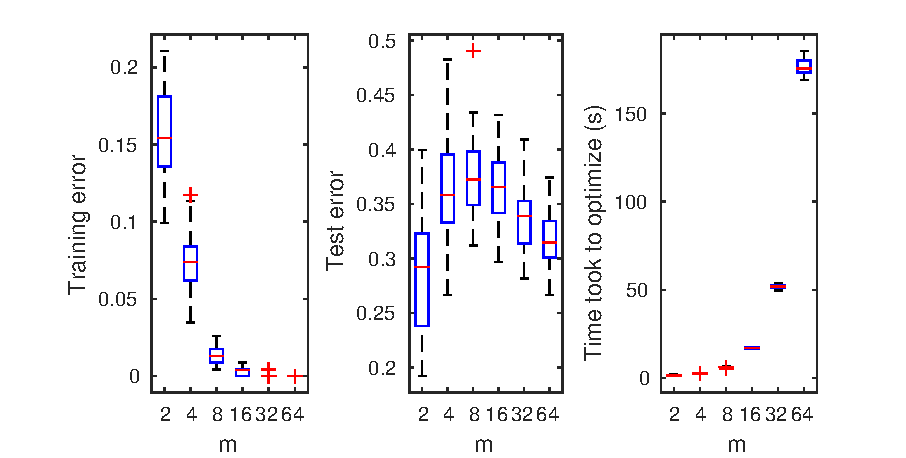
\includegraphics[width=\textwidth]{quasi_newton}
        \caption{Quasi-Newton}
    \end{subfigure}
    \begin{subfigure}{0.75\textwidth}
        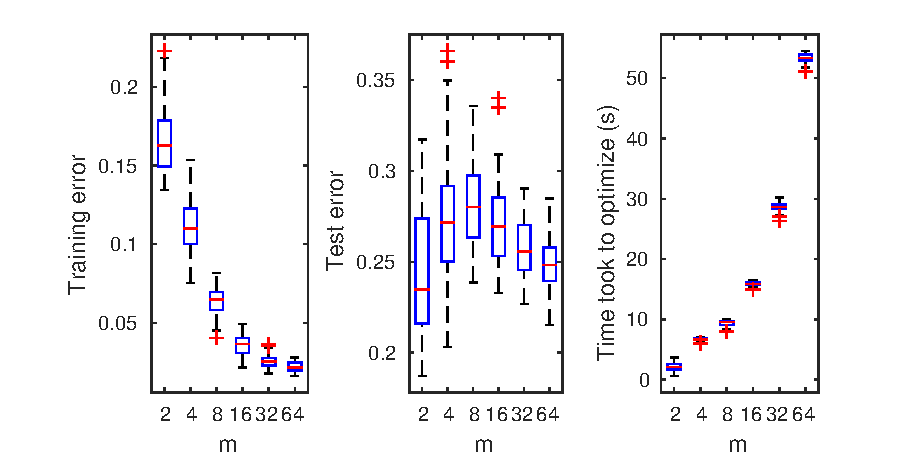
\includegraphics[width=\textwidth]{gradient_descent}
        \caption{Gradient Descent, step size = 0.1}
    \end{subfigure}
        \begin{subfigure}{0.75\textwidth}
        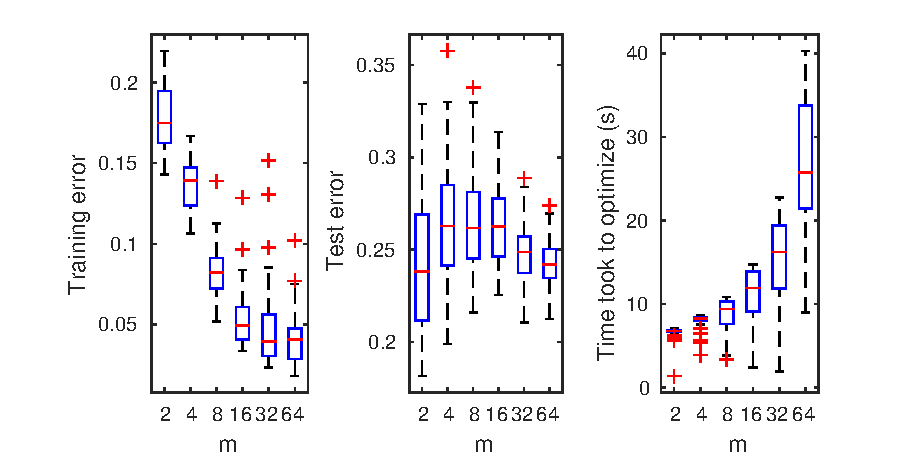
\includegraphics[width=\textwidth]{stochastic_gradient_descent}
        \caption{Stochastic Gradient Descent, step size = 0.1}
    \end{subfigure}
    \caption{Training error, test error and time took to optimize the objective for fitting the random Fourier representations onto the dataset \emph{SAheart}. The experiments were repeated 48 times with different initial values. The training and test set was split 50:50.}
    \label{SAheart}
\end{figure*}


\begin{figure}[h]
\centering
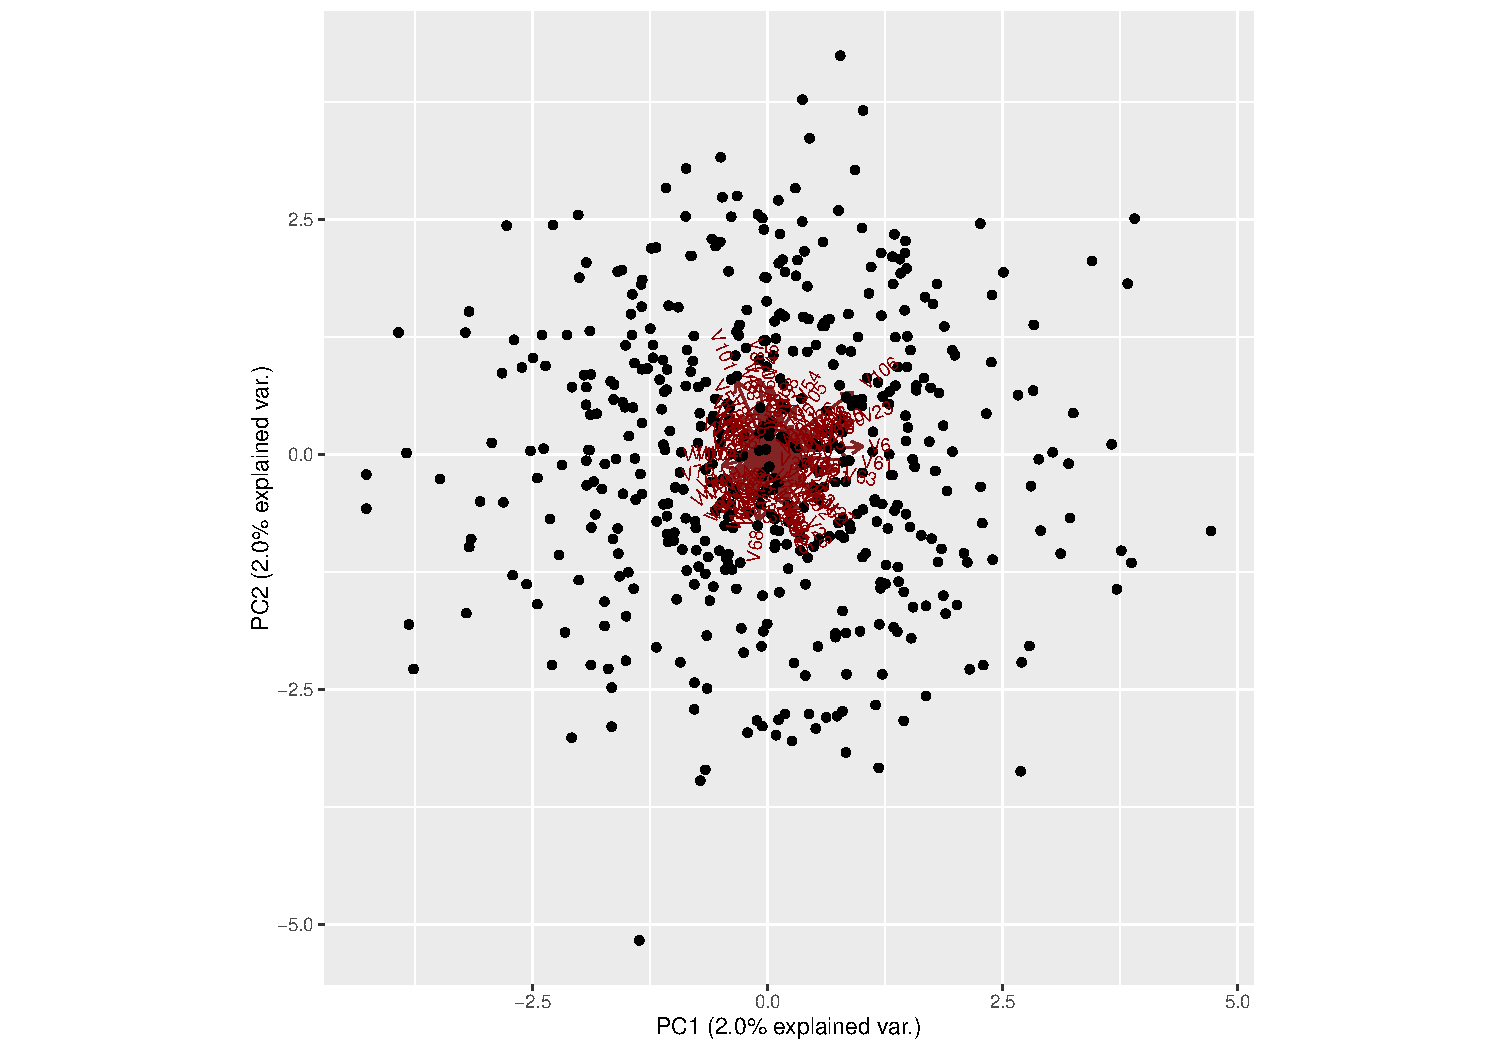
\includegraphics[width=15cm]{PCA_nn}
\caption{PCA of frequencies fitted using neural nets}\label{fig:PCA_nn}
\end{figure}

\begin{figure}[h]
\centering
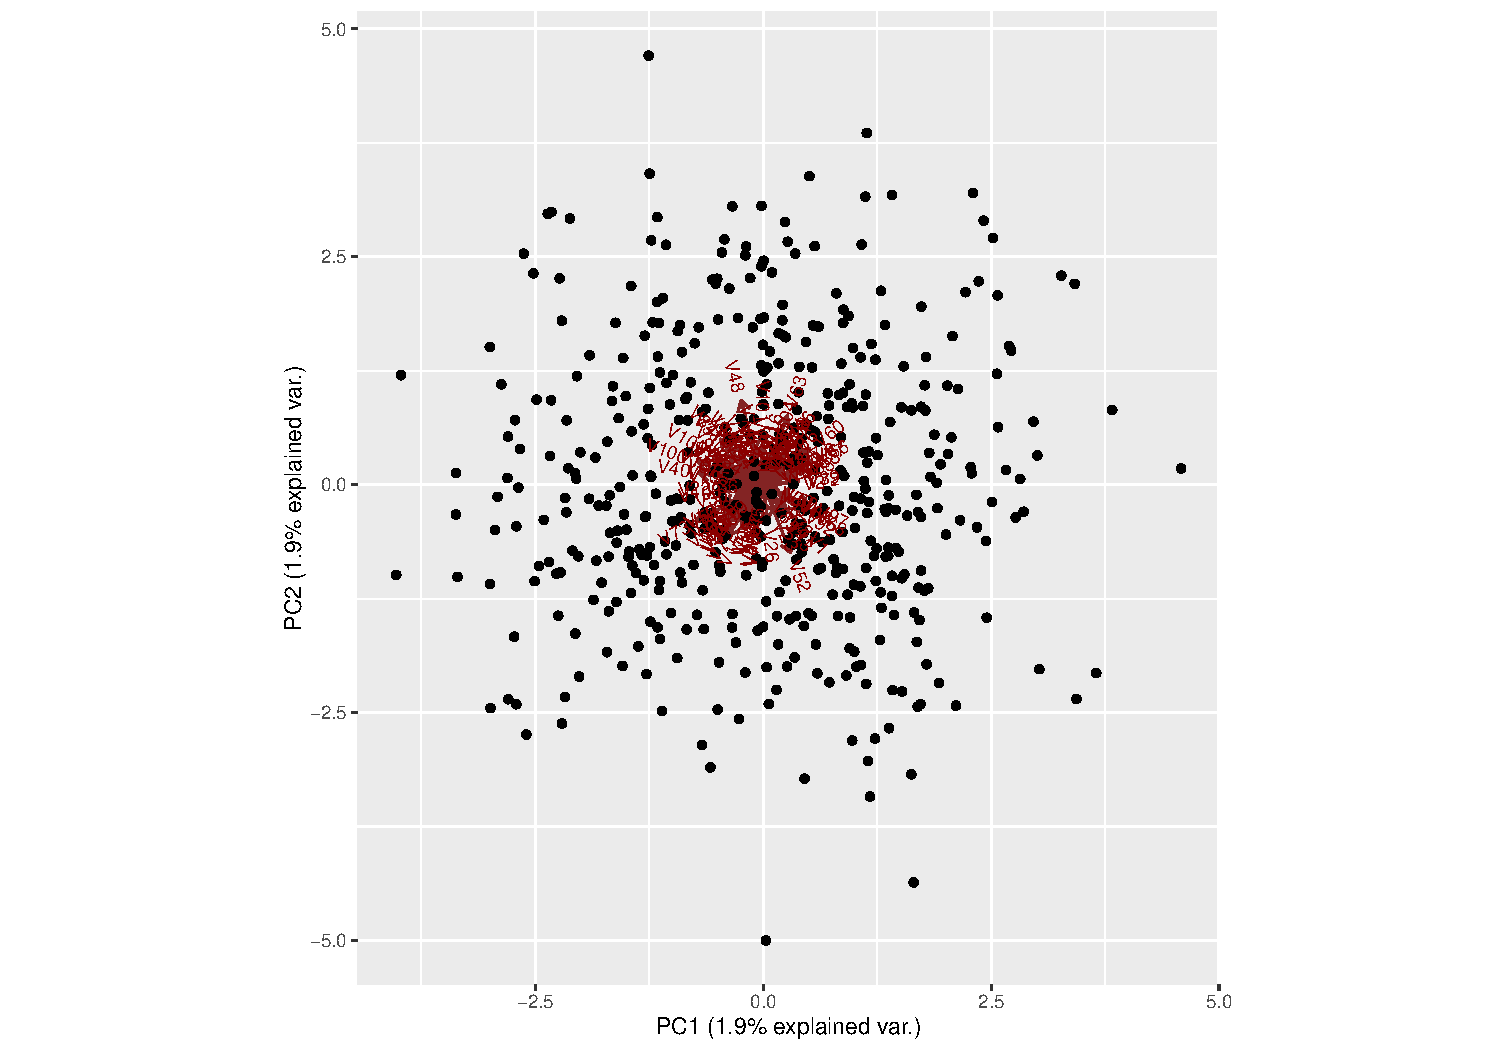
\includegraphics[width=15cm]{PCA_rff}
\caption{PCA of frequencies simulated at random for RFF}\label{fig:PCA_rff}
\end{figure}

\end{document}
